In this section, we demonstrate the results of \cref{thm:meas_cond,prop:gam_fam_cond} by numerically computing the conditioning of various spanning families.  In \cref{sec:expl_num}, we verify the bounds for the condition number of the exponential and near-flat mask local Fourier measurement systems studied in \cref{sec:exp_mask,sec:nearflat_mask}.  Additionally, we consider local Fourier measurement systems using a physically ``natural'' mask, where the illumination function is concentrated in the center and decays symetrically to the sides according to a Gaussian bell curve; although we have no theoretical guarantees for such a construction, conversations with crystallographers (in particular, the principal author of \cite{andrej2018battery}) have suggested that this is a realistic model, so we take a practical interest in its suitability for the algorithm proposed in \cref{ch:base_model}.  \Cref{sec:distvar_num} visualizes the propagation of variance studied in \cref{sec:dist_var} for particular instantiations of these same masks, suggesting that the condition number belies the typical level of noise magnification.  In \cref{sec:rand_fam}, we perform a Monte Carlo simulation to estimate the distribution of condition numbers among randomly generated local measurement systems, both general and Fourier%% , and in \cref{sec:span_fam_full} we replicate some of the experiments of \cref{sec:SparseMeasureMasks} with a variety of measurement systems to gauge the relative improvement in performance afforded by these better constructions
.

%In this section, we demonstrate the theory proven in the rest of this chapter with a few numerical experiments and examples of families of masks that satisfy the conditions to be spanning families, as established in \cref{thm:meas_cond,cor:gam_fam_span}.  In \cref{sec:reanalyze}, we confirm the existing results for the condition numbers of the measurement operators for Examples 1 and 2 in \cref{sec:MeasMatrix} by applying this theory to them.  In \cref{sec:num_ex}, we numerically compute the condition numbers for a few local Fourier measurement systems that seem intuitive (or practical), but whose condition numbers may be difficult to calculate theoretically.  Additionally, we run this experiment on randomly generated families of masks (both general and Fourier measurement systems) to illustrate the property of spanning families being ``generic,'' in the sense described in \cref{sec:span_fam_remarks}.

\subsection{Conditioning of Exponential and Near-Flat Masks}
\label{sec:expl_num}
Here, we make a numerical study of the conditioning of the local Fourier measurement systems analyzed in \cref{sec:reanalyze} to verify the tightness of the bounds we discovered in \cref{prop:exp_kappa,prop:spike_one}.  \Cref{fig:exp_kappa} shows two visualizations of $\kappa$ for the exponential mask $\gamma_i = a^i, i \in [\delta]$, which depends on $a, \delta$, and $d$.  The first, in \cref{fig:exptable}, shows a heatmap representing how $\kappa$ varies over $a$ and $\delta$ for a fixed value of $d = 32$.  Noticing the logarithmic scale on the colorbar, it's clear that choosing $a$ correctly is extremely important for having a decently conditioned system: once $\delta$ exceeds $14$ or so, there's a factor of greater than $10^2$ between the optimal condition number and the condition number for $a = 2$.  The black $\times$'s in the diagram represent the choice of $a, a_\delta$, recommended for each value of $\delta$ in \cref{prop:exp_kappa}, and we observe that the values of $a_\delta$ appear to track the optimal basin quite closely.

\begin{figure}
  \centering
  \begin{subfigure}[b]{.49\textwidth}
    \centering
    \includegraphics[width=\textwidth,trim={.4in 2.5in .8in 2.5in}]{figs/exptable32}
    \caption{$\log \kappa$ over $a$ and $\delta$, $d = 32$}
    \label{fig:exptable}
  \end{subfigure}
  \begin{subfigure}[b]{.49\textwidth}
    \centering
    \includegraphics[width=\textwidth,trim={.2in 2.5in 1in 2.5in}]{figs/expchart80}
    \caption{$\kappa$ over $\delta$; $d = 80$}
    \label{fig:expchart}
  \end{subfigure}        
  \caption{Condition number for exponential mask local measurement systems}
  \label{fig:exp_kappa}
\end{figure}

We confirm this intuition further in \cref{fig:expchart}, where we plot $\kappa$ vs.~$\delta$ for four distinct choices of $a$ as a function of $\delta$.  As described in the legend, the blue and red curves represent constant choices of $a$, the black curve represents an estimate of the optimal $\kappa$ (computed by performing an exhaustive search to a resolution of $1 / 128$ over $a \in (1, 2]$ for each $\delta$), and the black $\times$'s represent $\kappa(a_\delta)$, as in \cref{fig:exptable}.  This figure shows precisely the behavior we would expect if the bound of \eqref{eq:kap_est} were tight: for a fixed $a$, the condition number is asymptotically bounded by $C a^{\delta + 1}$,  which on a log scale becomes $\delta \log a + b$.  We see that, after about $\delta = 10$, both of the constant $a$ curves appear linear.  Of course, they intersect the ``optimal $a$'' curve when the optimal $a$ coincides with these constant choices, which may be judged by comparing with \cref{fig:exptable}.  The other interesting result is that this chart corroborates our expectation that the recommended choice $a_\delta$ is close to optimal: indeed, the $\kappa(a_\delta)$ marks are practically indistinguishable from the optimal $\kappa$ curve. %% (which was estimated to a resolution of $1/128$ by a linear search)
  We should expect this observation at least asymptotically in $\delta$, since our bound on $\kappa(a_\delta)$ is asymptotically tight: the value $a_\delta = (1 + \frac{4}{\delta - 2})^{1 / 2}$ optimizes the expression $\frac{a^{\delta + 2}}{(a^2 - 1)^2}$, which is an intermediate term in \eqref{eq:kapadel_approx}, and every inequality in \eqref{eq:kapadel_approx} is individually tight as $d$ and $\delta$ grow large.
  \begin{figure}
    \centering
    \begin{subfigure}[b]{.49\textwidth}
      \centering
      \includegraphics[width=\textwidth,trim={.4in 2.5in .8in 2.5in}]{figs/flattable}
      \caption{$\kappa$ over $a / \delta$ and $\delta$, $d = 6 \delta - 1$}
      \label{fig:flattable}
    \end{subfigure}
    \begin{subfigure}[b]{.49\textwidth}
      \centering
      \includegraphics[width=\textwidth,trim={.2in 2.5in 1in 2.5in}]{figs/flatchart}
      \caption{$\kappa$ over $\delta$, $d = 6 \delta - 1$}
      \label{fig:flatchart}
    \end{subfigure}
    
    \caption{Condition number for near-flat mask local measurement systems}
    \label{fig:flat_kappa}
  \end{figure}

In \cref{fig:flat_kappa}, we make a similar visualization of the conditioning of the near-flat mask measurement systems.  \Cref{fig:flattable} shows how $\kappa$ varies against $\delta$ and $a / \delta$, and we see that the recommended choice $a = 2 \delta - 1$ is quite suboptimal; one simple improvement suggested by the work in \cref{app:nearflat_more} is shown, where we take $a = 2 C \delta$ for $C \approx 0.217$, and the improvement is clear, although this choice still is not optimal (the optimal value of $a / \delta$ is plotted as $\times$'s).  \Cref{fig:flatchart} compares the condition number achieved by each of these three selections of $a$, where again the optimal value is obtained, to a resolution of $1 / 128$, by a linear search.  As expected, the two choices of $a$ which are affine in $\delta$ produce condition numbers roughly linear in $\delta$, and the optimal value doesn't appear to be of a lower order.  At any rate, the guarantees provided in \cref{prop:spike_one,prop:nearflat_more} are validated, at least in upper bounding the growth of $\kappa$ with the size of the problem.

\begin{figure}
  \begin{subfigure}[b]{.49\textwidth}
    \centering
    \includegraphics[width=\textwidth,trim={.4in 2.5in .8in 2.5in}]{figs/gaustable}
    \caption{$\kappa$ over $k$ and $\delta$, $d = 6 \delta - 1$}
    \label{fig:gaustable}
  \end{subfigure}
  \begin{subfigure}[b]{.49\textwidth}
    \centering
    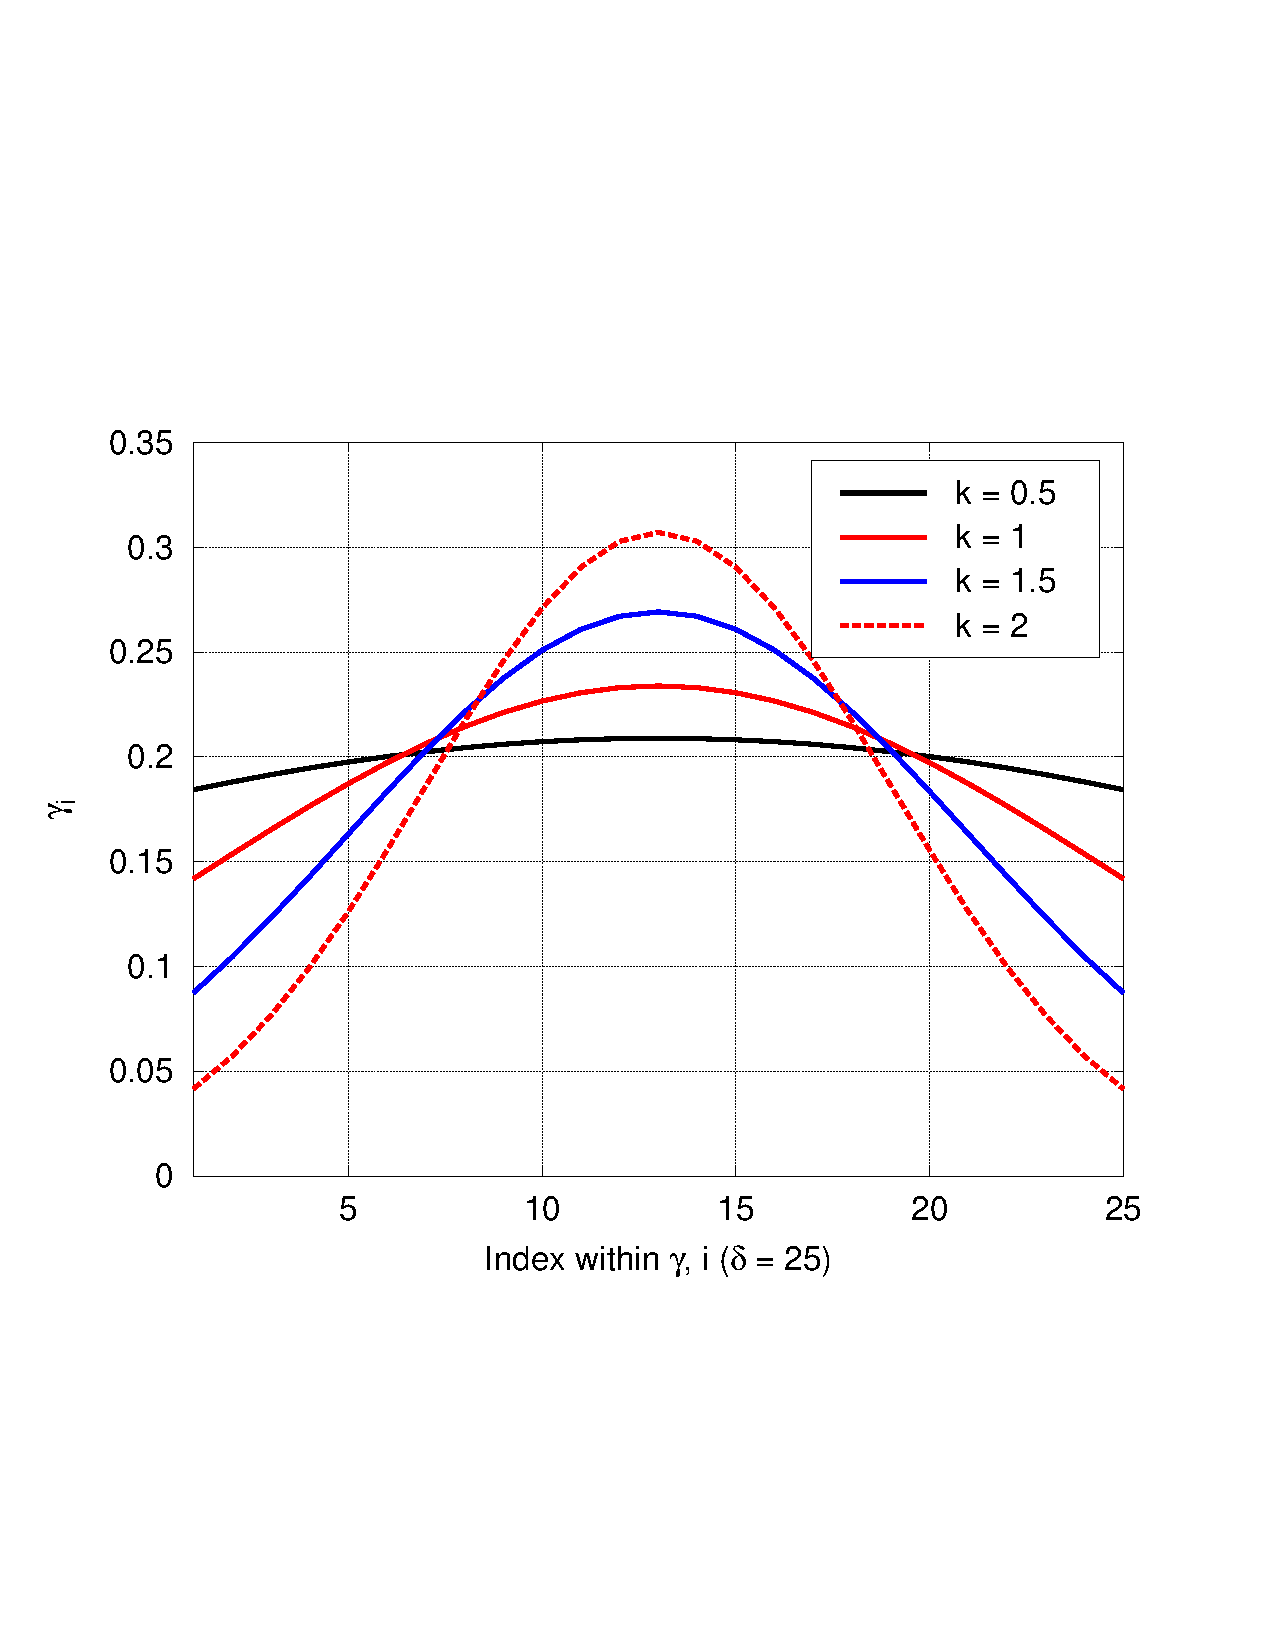
\includegraphics[width=\textwidth,trim={.4in 2.5in .8in 2.5in}]{figs/gauschart}
    \caption{$\gamma$ for different values of $k, \delta = 25$}
    \label{fig:gausmask}
  \end{subfigure}
  \caption{Gaussian illumination masks}
  \label{fig:gaustables}
\end{figure}

\Cref{fig:gaustable} gives a heatmap of the condition number for the linear system corresponding to a ``natural'' illumination function, where $\gamma \in \Rd$ is defined by \[\gamma_i = \begin{piecewise} C \ee^{- \frac{(i - \mu)^2}{2 \sigma^2}} & i \in [\delta] \\ 0 & \ow \end{piecewise}\] with $\mu = \frac{\delta + 1}{2}$ (so that the illumination is concentrated at the center of the mask), $C$ chosen such that $\norm{\gamma}_2 = 1$, and $\sigma = \frac{\delta - 1}{2 k}$, where $k$ is the width of $[\mu, \delta]$ in standard deviations.  We consider this choice of $\gamma$ to be natural in the sense that it roughly models the brightness of a laser beam which is pointed at the center of our window $[1, \delta]$.  To visualize how concentrated or spread out are the masks under consideration in \cref{fig:gaustable}, $\gamma$ is plotted for a few sample values of $k$ in \cref{fig:gausmask}.  Unfortunately, though, as we can see in \cref{fig:gaustable}, the conditioning of masks of this variety is overwhelmingly unstable, with little to no recognizable pattern in the dependence of $\kappa$ on $k$ and $\delta$.  In many spots, varying $\delta$ by $1$ (liable to occur as an artifact of discretization) or changing $k$ by $\approx 0.05$ (not a large change; see \cref{fig:gausmask}) can worsen $\kappa$ by multiple orders of magnitude.  As $\kappa$ is smooth neither in $\delta$ nor $k$, these types of masks appear to be unsuitable for \cref{alg:phaseRetrieval1}.

\subsection{Numerical Distribution of Variance}
\label{sec:distvar_num}

\begin{figure}
  \centering
    \includegraphics[width=.7\textwidth,trim={.4in 2.5in .8in 2.5in}]{figs/realvar}
  \caption{Actual variance $\abs{s_m}_1$ along each diagonal for exponential, flat, and Gaussian masks}
  \label{fig:realvar}
\end{figure}

\Cref{fig:realvar,fig:distvar64} illustrate the results of \cref{prop:var_dist} in section \cref{sec:dist_var}.  The experiment run for \cref{fig:distvar64} was to fix a family of masks $\{m_j\}_{j \in [D]}$ and solve the linear system $\Ac(X) = y$ for several pseudo-randomly generated vectors of measurements $y \sim \Nc(0, I_{dD})$, and then calculate and plot the sample variance for each entry of $X = \Ac^{-1}(y)$.  We repeated this for one particular realization (fixing $d, \delta$, and parameters) of the exponential, near-flat, and Gaussian masks discussed in \cref{sec:expl_num}; we will refer to these three mask vectors as $\gamma_{\rm exp}, \gamma_{\rm flat},$ and $\gamma_{\rm gauss}$ for the remainder of this section.  The figure captions in \cref{fig:distvar64} show the parameters $d, \delta$, and $a$ (or $k$) used for each experiment.  These heatmaps display $d \times d$ grids, where the $(i, j)\th$ pixel represents the sample variance of $X_{ij}$, and the perfectly blue bands observed are simply the parts of $X$ that are ``zeroed out'' by the $T_\delta(X)$ restriction.  First of all, we remark the scales used on each of these graphs: the exponential and near-flat masks exhibit variance at similar orders of magnitude, while the Gaussian measurement system (using masks from \cref{fig:gausmask} with $a = 2$) produces variance on the entries that is several orders of magnitude higher.  This is absolutely an issue with the conditioning of the Gaussian system, since our design of the masks has given us \[\norm{\gamma_{\mathrm{exp}}}_2^2 = 191.65, \norm{\gamma_{\rm flat}}_2^2 = 78.226, \norm{\gamma_{\rm gauss}}_2^2 = 1,\] so unit-variance noise on the $\gamma_{\rm gauss}$ measurements ought to be no more than $200x$ as significant as similar noise on the exponential or flat measurements, by a rough Cauchy-Schwarz estimate: \[\Ac(x x^*)_{(\ell, j)} = \abs{\inner{x, S^\ell m_j}}^2 \le \norm{\gamma}_2^2 \norm{x}_2^2.\]  And this result -- where the Gaussian masks are far less competitive -- is unsurprising, considering the horrendous stability observed in \cref{fig:gaustable}.

More interesting, then, is to view how the variance is distributed over the diagonals when using the exponential and flat masks.  Referring to \cref{fig:expvar64,fig:flatvar64}, the main diagonal appears to have the most accurate entries in both cases.  For the flat masks, the off-diagonal entries of $\Ac^{-1}(y)$ appear to have roughly equal uncertainty, while the entries almost monotonically increase in variance as you get farther away from the main diagonal with the exponential masks.  Interestingly, the penultimate off-diagonal has the greatest variance with the exponential masks.  These observations are confirmed in \cref{fig:realvar}, where we have used \cref{prop:var_dist} to calculate the \emph{actual} variance (specifically, we calculate $\abs{s_m}_1$ as a function of $m \in [\delta]_0$) of the entries of $\Ac^{-1}(y)$) for all three of these measurement systems.  We emphasize that the Gaussian variance curve uses the logarithmic scale on the right side of the graph, while the other two curves use the linear scale on the left.

One useful feature of this analysis is that it suggests that randomly-distributed noise (in the sense that $y_{(\ell, j)} = \abs{\inner{x, S^\ell m_j}}^2 + \eta_{(\ell, j)}$ with $\eta_{(\ell, j)} \iid \Nc(0, \sigma^2)$) will typically cooperate with the magnitude estimation step in line 4 of \cref{alg:phaseRetrieval1}.  In particular, if $x_0 \in \C^d$ is the ground truth and $X = \Ac^{-1}(y)$ is our estimate of $X_0 = T_\delta(x_0 x_0^*)$, then we might expect $\norm{\diag(X - X_0)}_1$ to be considerably smaller than $d^{1 / 4} \norm{X - X_0}_F$; considering \cref{lem:diag_mag_diff} along with these numerical results, this suggests that typical noise will not be adversarial to our simple magnitude estimation technique.

%% \begin{figure}
%%   \centering
%%   \begin{subfigure}[b]{.49\textwidth}
%%     \centering
%%     \includegraphics[width=\textwidth,trim={.4in 2.5in .8in 2.5in}]{figs/expvar64}
%%     \caption{Exponential masks. \\ $d = 64, \delta = 16, a = a_\delta \approx 1.134$}
%%     \label{fig:expvar64}
%%   \end{subfigure}
%%   \begin{subfigure}[b]{.49\textwidth}
%%     \centering
%%     \includegraphics[width=\textwidth,trim={.4in 2.5in .8in 2.5in}]{figs/flatvar64}
%%     \caption{Near-flat masks.\\  $d = 64, \delta = 16, a = 2 C \delta \approx 6.952$}
%%     \label{fig:flatvar64}
%%   \end{subfigure}
%%   \begin{subfigure}[b]{.49\textwidth}
%%     \centering
%%     \includegraphics[width=\textwidth,trim={.4in 2.5in .8in 2.5in}]{figs/gausvar64}
%%     \caption{Natural/gaussian masks.\\  $d = 63, \delta = 16, a = 2$}
%%     \label{fig:gausvar64}
%%   \end{subfigure}
%%   \caption{Variance of entries of $X = \Ac^{-1}(y)$ for $y \sim \Nc(0, I_{dD})$, $N = 64$ samples}
%%   \label{fig:distvar64}    
%% \end{figure}

\begin{figure}
  \centering
  \begin{subfigure}[b]{.49\textwidth}
    \centering
    \includegraphics[width=\textwidth,trim={.4in 2.5in .8in 2.5in}]{figs/expvar512}
    \caption{Exponential masks. \\ $d = 64, \delta = 16, a = a_\delta \approx 1.134$}
    \label{fig:expvar64}
  \end{subfigure}
  \begin{subfigure}[b]{.49\textwidth}
    \centering
    \includegraphics[width=\textwidth,trim={.4in 2.5in .8in 2.5in}]{figs/flatvar512}
    \caption{Near-flat masks.\\  $d = 64, \delta = 16, a = 2 C \delta \approx 6.952$}
    \label{fig:flatvar64}
  \end{subfigure}
  \begin{subfigure}[b]{.49\textwidth}
    \centering
    \includegraphics[width=\textwidth,trim={.4in 2.5in .8in 2.5in}]{figs/gausvar64}
    \caption{Natural/gaussian masks.\\  $d = 63, \delta = 16, k = 2$}
    \label{fig:gausvar512}
  \end{subfigure}
  \caption{Sample variance of entries of $X = \Ac^{-1}(y)$ for $y \sim \Nc(0, I_{dD})$, $N = 512$ samples}
  \label{fig:distvar64}    
\end{figure}
